\documentclass[11pt]{article}
\usepackage{amsmath, amssymb, amscd, amsthm, amsfonts}
\usepackage{graphicx}
\usepackage{subcaption}
\usepackage{wrapfig}

\graphicspath{ {./Images/} }
\usepackage{hyperref}

\oddsidemargin 0pt
\evensidemargin 0pt
\marginparwidth 40pt
\marginparsep 10pt
\topmargin -20pt
\headsep 10pt
\textheight 8.7in
\textwidth 6.65in
\linespread{1.2}

\title{Trust Region Policy Optimization - Implementation}
\author{Pietro Nardelli \\ \\
        Master's Degree in Artificial Intelligence and Robotics \\
        Department of Computer, Control and Management Engineering \\
        Sapienza University of Rome}

\date{January 2020}

\begin{document}

\maketitle

\section{Introduction}
Trust Region Policy Optimization is an algorithm that make several
approximations to a theoretical iterative procedure for optimizing policies with
guaranteed monotonic improvement. Despite its approximations that deviate from
the theory, TRPO tends to give monotonic improvement, while little tuning of
hyperparameters. This algorithm is effective for optimizing large nonlinear
policies such as neural networks. The algorithm has been tested on two different
openAI gym environments. Gym library is a collection of test problems that can
be used to test reinforcement learning algorithms.

\section{Environments}

\subsection{MountainCarContinuous-v0}
An underpowered car must climb a one-dimensional hill to reach a target. The
action (engine force applied) is allowed to be a continuous value.
The target is on top of a hill on the right-hand side of the car. If the car reaches it or goes beyond, the episode terminates.
\\
On the left-hand side, there is another hill. Climbing this hill can be used to
gain potential energy and accelerate towards the target. On top of this second
hill, the car cannot go further than a position equal to -1, as if there was a
wall. Hitting this limit does not generate a penalty.
\\
The observations are CarPosition and CarVelocity and the only action permits to
push the car on the left (negative values) or on the right (negative values).
\\
Reward is 100 for reaching the target of the hill on the right hand side,
minus the squared sum of actions from start to goal.

This reward function raises an \textbf{exploration challenge}, because if the agent does
not reach the target soon enough, it will figure out that it is better not to move,
and won't find the target anymore.
\\
To consider the problem solved, the reward should be over 90.


\subsection{LunarLanderContinuous-v0}
A lunar lander is a spacecraft designed to land on the Moon. Landing pad is always at coordinates
(0,0). Reward for moving from the top of the screen to landing pad and zero speed is about 100-140
points. If lander moves away from landing pad it loses reward back. Episode finishes if the lander
crashes or comes to rest, receiving additional -100 or +100 points. Each leg ground contact is +10.
Firing main engine is -0.3 points each frame (fuel is infinite). Solved is 200 points. Action is two
real values vector from -1 to +1. First controls main engine, [-1,0] off, [0,1] throttle from 50\%
to 100\% power, Second value [-1.0,-0.5] fire left engine, [0.5,1.0] fire right engine, [0.5,0.5]
off.
\begin{figure}[h!]
        \centering
        \begin{subfigure}[b]{0.4\linewidth}
                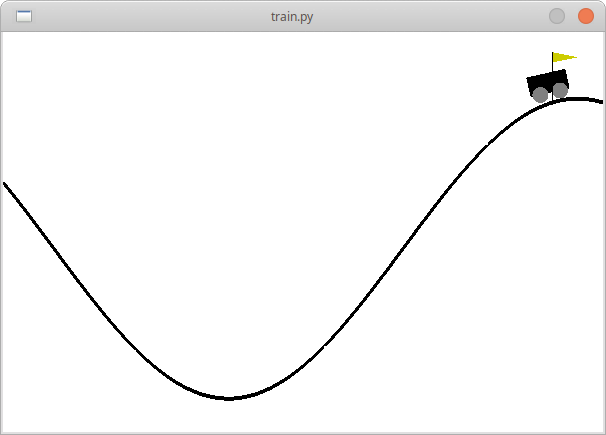
\includegraphics[width=\linewidth]{mountain_screen}
                \caption{}
        \end{subfigure}
        \begin{subfigure}[b]{0.4\linewidth}
                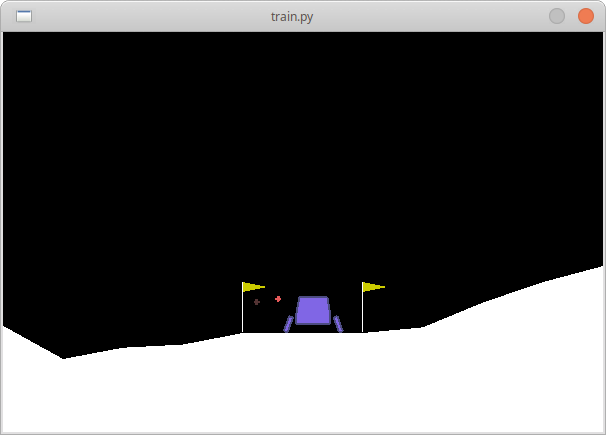
\includegraphics[width=\linewidth]{lunar_screen}
                \caption{}
        \end{subfigure}

        \caption{ Both the environments just described. (a) MountainCarContinuous-v0 when reaching the goal position.(b) LunarLanderContinuous-v2 when reaching the landing pad.}
        \label{fig:screens}
\end{figure}

\section{TRPO algorithm}\label{section-trpo}
TRPO Trust Region Policy Optimization is based on the Minorize-Maximization (MM)
algorithm. The MM algorithm can guarantee that any policy updates always improve the
expected rewards. This is achived iteratively by maximizing a lower bound function
approximating the expected reward locally, as we can see in figure \ref{fig:functions1},
(with $\pi$ denote a stochastic policy and $\eta(\pi)$ denote its expected discounted
reward). After each iteration of the MM algorithm the policy keeps improving. Since there
is only finite possible policy, our current policy will eventually converge to the local
or the global optimal.
\begin{figure}[t]
        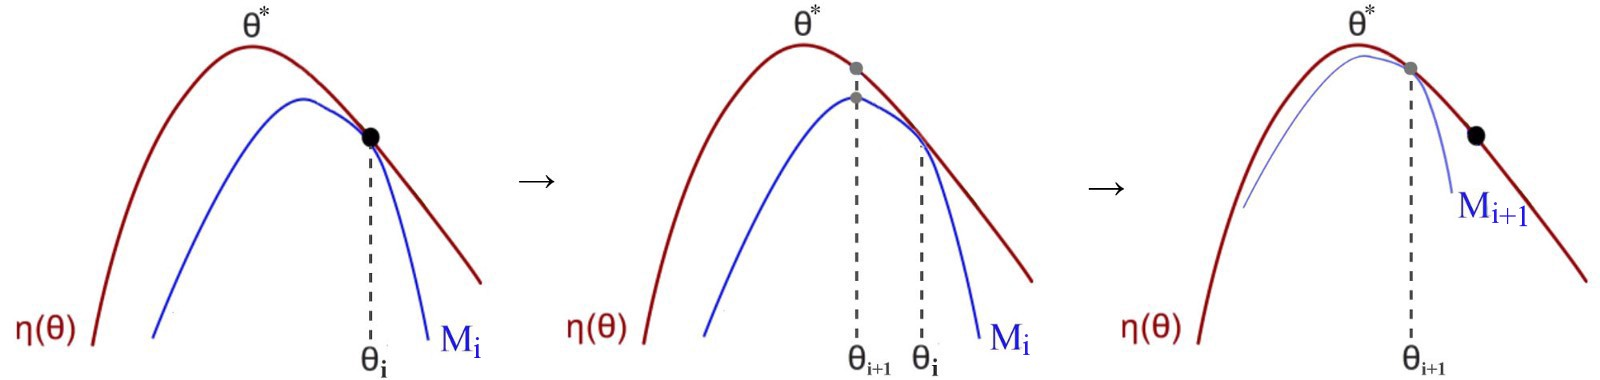
\includegraphics[width=15cm]{functions1}
        \centering
        \caption{Minorization-Maximization algorithm where M is a lower bound for $\eta$
        (surrogate function). Eventually our guess will converge to the optimal policy but
        to make this work $M$ should be easier to optimize than $\eta$ (in fact M is
        usually approximating to a quadratic equation that is a convex function). }
        \label{fig:functions1}
\end{figure}

The evolution of this kind of algorithm is called Trust Region Policy Optimization (TRPO),
which uses a constraint on the Kullback–Leibler (KL) divergence rather than a penalty to
robustly allow large updates. The KL divergence is a measure of how one probability
distribution $P$ is different from a second probability distribution $Q$ that is a
reference for the first one: $D_{KL}(P||Q)$.

\begin{figure}[t]
        
\includegraphics[width=15cm]{functions2}
        \centering
        \caption{In practice, if penalty coefficient is included in the objective function,
        the step size will be very small, leading to long training time.
        Consequently, a constraint on the KL divergence is used to allow a larger step size
        while guarantee robust performance.
        }
        \label{fig:functions2}
\end{figure}
In fact, supposing that we used a penalty coefficient C (that is recommended by theory),
the step sizes would be very small (fig. \ref{fig:functions2}). One way to take larger
steps in a robust way is to use a constraint on the KL divergence between new policy and
old policy (trust region constraint):
\begin{equation}
        \begin{split}
        maximize_{\theta} \ L_{\theta_{old}}(\theta)
        \\ \label{eq:1}
        subject \  to \ D_{KL_{max}}(\theta_{old}, \theta) \leq \delta
        \end{split}
\end{equation}
Since $\eta$ is hard to optimized, $L$ is a local approximation to $\eta$. While it's
motivated by the theory, this problem is impractical to solve due to large number of
constraints. Unfortunately, it is not solvable as there are a infinitely large number of
states: we can use a heuristic approximation which considers the avarage KL divergence
$\bar{D_{KL}}$. Our optimization problem in equation (\ref{eq:1}) is exactly equivalent to
the following one (written in terms of expectations, replacing some terms, under the
assumption that $D_{KL}(\theta|| \tilde{\theta}) :=
D_{KL}(\pi_{\theta}||\pi_{\tilde{\theta}})$):

\begin{equation}
        \begin{split}
        maximize_{\theta} \ E_t\Big[\frac{\pi_{\theta}(a_t, s_t)}{\pi_{\theta_{old}}(a_t, s_t)}A_t\Big]
        \\ \label{eq:2}
        subject \  to \ D_{KL_{max}}(\theta_{old}, \theta) \leq \delta
        \end{split}
\end{equation}
The advantage function $A_{\pi} = Q_{\pi}(s, a) - V_{\pi}(s)$ is the difference between
state-action value function and value function. We can prove that any policy update $\pi
\rightarrow \tilde{\pi}$ that has a nonnegative expected advantage at every states is
guaranteeed to increase the policy performance $\eta$, or leave it constant in the case
that the expected advantage is zero everywhere. Intuitively, we can think of it as
measuring how good the new policy is with regard to the average performance of the old
policy. However, in the approximate setting, it will typically be unavoidable, due to
estimation and approximation error, that there will be some state s for which the expected
advantage is negative.
The objective function is also called a \textbf{surrogate objective function} as it contains a
probability ratio between current policy and the next policy. The subset of region lies
within the constraint is called \textbf{trust region}. As long as the policy change is reasonably
small, the approximation is not much different from the true objective function By
choosing the new policy parameters which maximizes the expectation subject to the KL
divergence constraint, a lower bound of the expected long-term reward $\eta$ is guaranteed.
In the trust region, we limit our search within a region controlled by $\delta$.
\\
A practical algorithm could be:

\begin{enumerate}
        \item Use a procedure to collect a set of state-action pairs.
        \item By averaging over samples, construct the estimated objective and constraint
        in equation \ref{eq:2}.
        \item Approximately solve this contrained optimization problem to update the
        policy's parameter vector $\theta$.

\end{enumerate}
The third point has been developed by the author with a conjugate gradient algorithm followed
by a line search, or in other words, compute a search direction and perform a line search
in that direction. The search direction is computed by approximately solve the equation
$Ax = g$ where $A$ is the Fisher information matrix (part of the KL divergence). Given
that this matrix is costly in large-scale problems, the conjugate gradient allows us to
approximately solve this equation without forming the matrix itself. Having computed the
search direction, it's necessary to use a line search to ensure
improvement of the surrogate objective and satisfaction of the KL divergence constraint.
\\
The real difference between gradient descent and conjugate gradient is that the
latter finds a search direction every time that is A-orthogonal (conjugate) to all previous
directions, so it would not undo part of the movement done previously (as we can see in fig. \ref{fig:gradient}).
As far as the author specifies that this is an efficient method to solve the problem, it's
really hard to implement practically. Given this difficulties in the implementation, I've
decided to solve the constraint optimization problem (eq. \ref{eq:2}), using an
handcrafted solution which uses gradient descent, even if it is not the most efficient
solution. 
The next section will explain the implementation choices for the algorithm.
\section{Implementation}
The algorithm as described in figure \ref{fig:pseudocode} has been developed using Python
3 and TensorFlow 2 as framework.

It has been used the single-path method in which a set of trajectories is generated via
simulation of the policy from $s_0$ for some number of timesteps.


\begin{wrapfigure}{r}{0.5\textwidth}
        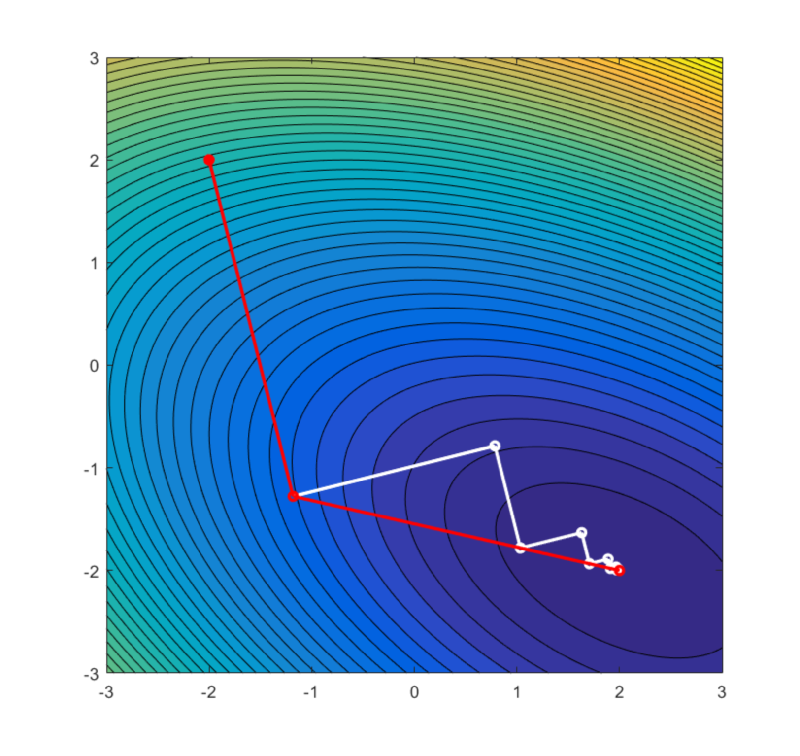
\includegraphics[width=0.4\textwidth]{gradient}
        \centering
        \caption{Difference between conjugate gradient (red line) and gradient descent
        (white line). Conjugate gradient can reach the minimum point of
        the function in less steps.}
        \label{fig:gradient}
\end{wrapfigure}
The advantage requires the value function that is approximated through a neural network.
The inputs of this neural network are the observations and the estimation has been made
with Mean Squared Error (MSE). Another fundamental neural network that has to be
implemented is the policy. Given a particular observation the policy neural network will
returns the means and log variance, composing a Gaussian distribution from which we can
sample the right action to choose. Anyway, to permits to the agent to make exploration (as
well as exploitation) $\epsilon$-greedy method has been implemented: the action to choose
at each state can be randomly selected with a probability $\epsilon=0.2$ 
\\
The policy network has been optimized with gradient descent on a loss function that is the negate of
our objective function from the equation (\ref{eq:2}). For each iteration, the policy has
to be trained (updated) for several epochs and for each epoch it's necessary to check if
$D_{KL} \leq \delta$. If this condition is not respected, then the constraint is not
either: the previous state (weights) of the neural network would be loaded in order to respect the
contraint. As we said in the previous section, this handcrafted method has been made to
find a trade-off between complexity and efficiency for the TRPO algorithm. \\
Altough theorically the constraint is respected, given the approximation of the value
function, it's not possible to obtain a positive advantage everytime. For this reason, as
we will see in the plots in the next paragraph, the policy will have monotonic improvement
overall only.
\\
The training of the policy has to be done each time over all the trajectories of a batch.
The batch size $bs$ has been set to 5 for memory reason.
Among the most important implementation choices, besides those already mentioned, there are:
\begin{itemize}
        \item Discount factor $\gamma$: is a value between 0 and 1 that tells how
        important future rewards are to the current state. This is set to 0.995.
        \item D-KL target value $\delta$: this is the upper value of the constraint.
        \item Policy learning rate $lr$: this is the learning rate of the policy neural
        network. This has to be chosen carefully otherwise the convergence would never be
        obtained. Empirically we can chose this value as the one that allow the policy to
        train for at least (on avarage) 10 epochs.
\end{itemize}


\begin{figure}[t]
        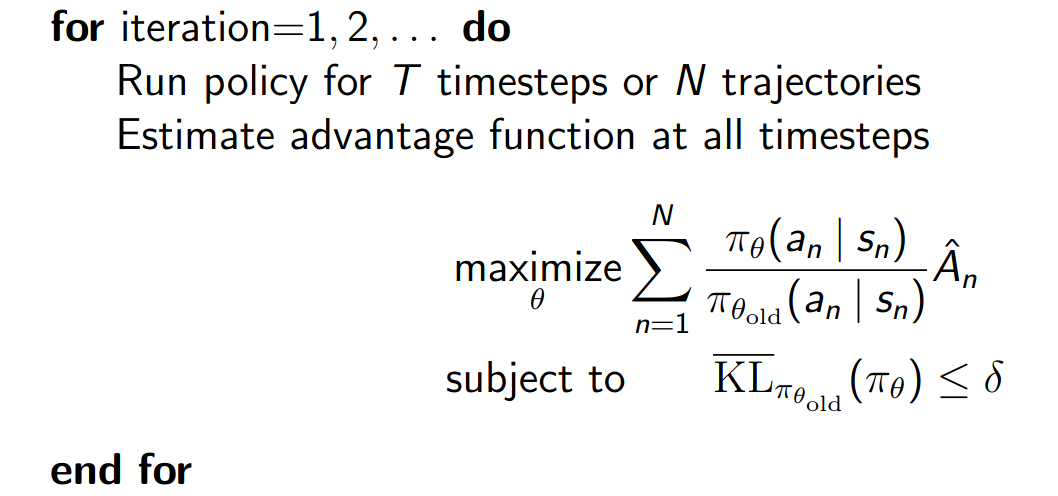
\includegraphics[width=9cm]{pseudocode}
        \centering
        \caption{Pseudocode for TRPO algorithm.}
        \label{fig:pseudocode}
\end{figure}

\section{Results}
Various tests have been made, tuning the parameters of the algorithm. All the previous
results for the most important parameters are valid in both the environment. Subsequent to
the completion of tuning, the results have been obtained training each agent for a
sufficient quantity of episodes. 
\subsection{MountainCarContinuous-v0}
For the mountain car environment is necessary to use $lr = 3 \cdot 10^{-4}$. This permits
to solve the problem (90 score) in about 500 episodes. As we can see in fig
\ref{fig:plots}a the agent for at least 200 episodes is training its policy to increase
rewards but without the exploration provided with $\epsilon$-greedy parameter, it wouldn't
be easy to reach the flag. After its positive reward, the agent obtain an exponentially
increase in rewards until it's near to solve the problem. 
It's possible to test this agent on its environment with the saved model in
\textit{"models/mountain.tf"} using the script \textit{test.py}.
\subsection{LunarLanderContinuous-v2}
For the lunar lander environment an improvement is possible with $lr = 5 \cdot 10^{-5}$ while
keeping all the parameters set for the previous environment. As we can see in
\ref{fig:plots}b, the agent will increase generally its performance but it requires more
than double of the episodes to reach a good behaviour, respect to mountain car environment. Further improvements
can be probably done to this problem tuning other parameters in addition to $lr$. It's possible to
test this agent on its environment with the saved model in \textit{"models/lunar.tf"}
using the script \textit{test.py}.

\begin{figure}[h!]
        \centering
        \begin{subfigure}[b]{0.7\linewidth}
                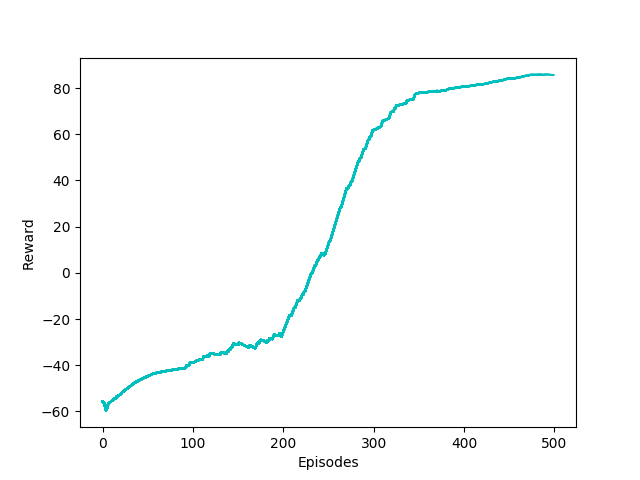
\includegraphics[width=\linewidth]{mountain_plot}
                \caption{}
        \end{subfigure}
        \begin{subfigure}[b]{0.7\linewidth}
                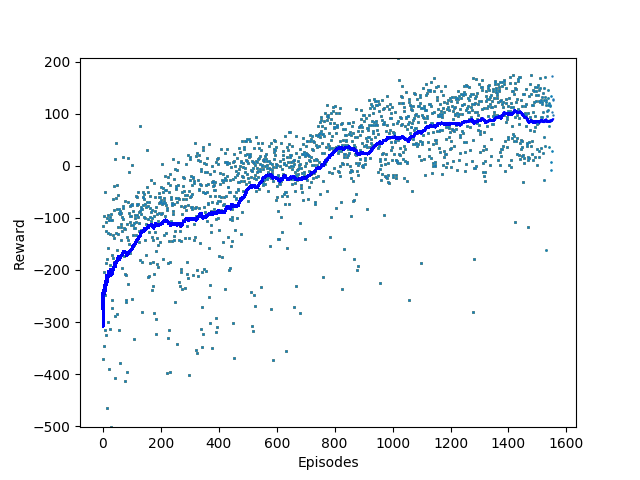
\includegraphics[width=\linewidth]{lunar_plot}
                \caption{}
        \end{subfigure}

        \caption{ Learning curves avaraged across five runs. 
                The environments in which the agent operates are 
                (a) MountainCarContinuous-v0 and (b) LunarLanderContinuous-v2.
                In the last environment it has been showed (as a scatter plot) the score
                for each episode}
        \label{fig:plots}
\end{figure}

\end{document}
